\chapter{Summary}
\label{cha:summary}

Conducted experiments show a gap between JavaScript and C++ performance. Significant language design differences result in code that is often easier to write but also easier to abuse. Benchmarks show differences between 15\% and 100\% overhead for correctly designed JavaScript code and over 500\% for incorrect patterns.  Considering Moore's law stating that computers double speed every 18 months it safe to say that JavaScript is very close to being suitable for any type of development. Recent projects varying from server side solutions\footnote{http://nodejs.org/}\footnote{http://googlecreativelab.github.io/coder/} to hardware developer boards\footnote{http://www.espruino.com/} are proving it. From the perspective of game development, it is unlikely at the time of writing that AAA game may be created to run in browser. However, growing segments of casual, independent and social games are already targeting web as a platform.

\begin{figure}[h!]
  \caption{Game created with ImpactJS}
  \label{img:impactjs}
  \centering
	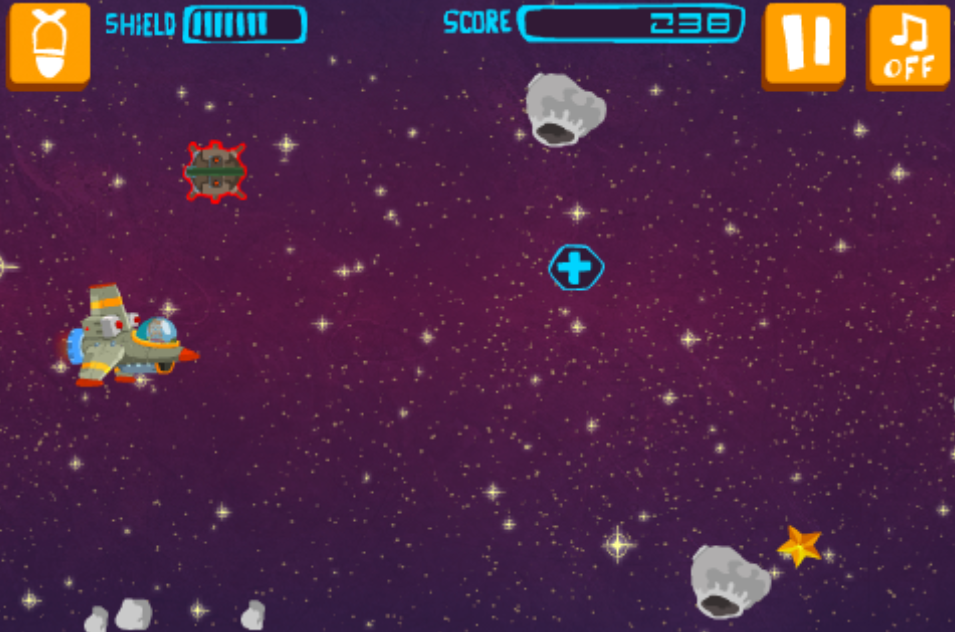
\includegraphics[width=12cm]{summary/impactjs.png}
\end{figure}

Multiple open-source and commercial game engines are created lately. Examples worth mentioning are ImpactJS\footnote{http://impactjs.com/}, Turbulenz\footnote{http://biz.turbulenz.com/turbulenz} and Isogenic Engine\footnote{http://www.isogenicengine.com/}.


\begin{figure}[h!]
  \caption{Game created with Isogenic Engine}
  \label{img:isogenic}
  \centering
	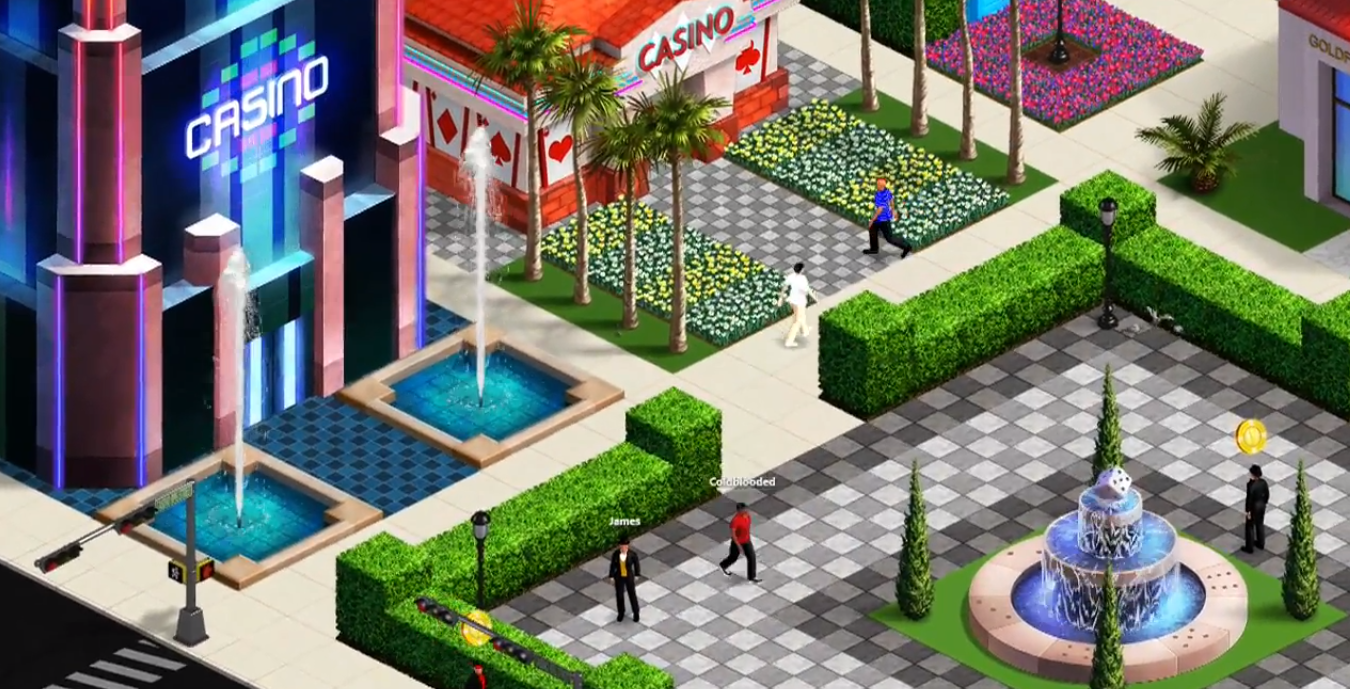
\includegraphics[width=12cm]{summary/isogenic.png}
\end{figure}

Very important and growing sector are interactive 3D arts with two major targets - music videos and commercials. They are uniquely available only in browsers as a very viral extensions of normal marketing. On of first occurrences of this use of technology was video for Rome group: "3 dreams of black"\footnote{http://www.ro.me/}. Project allows to move the camera while animated 3D story is rendered for music. After movie is over user is allowed to create 3D models that are later incorporated into experiences of next people watching. This way interactions and social element are enabled in what used to be one-way transmission of art form. 

\begin{figure}[h!]
  \caption{Screenshot from "3 dreams of black"}
  \label{img:rome}
  \centering
	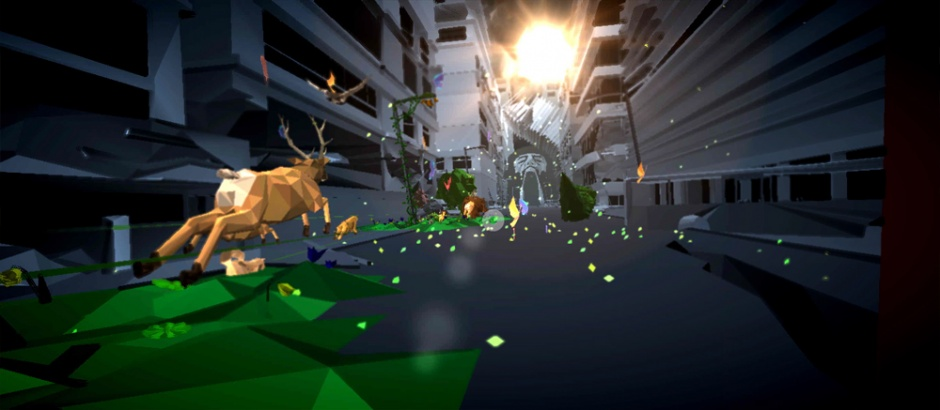
\includegraphics[width=12cm]{summary/rome.jpg}
\end{figure}

\section{Encountered environment limitations}
\label{sec:limitations}

\section{Browser advantages}
\label{sec:advantages}

\section{Recommended techniques}
\label{sec:recommended}

\section{Final thoughts}
\label{sec:final} 
